\section{Motivation} 
\label{sec:motivation}
\paragraph{}
Spark-like big-data computing runtimes shift data storage locations from
disks to memory, thus create excessive pressure on the current memory
subsystems.  We believe that current memory subsystems are not well
suited to handle spikes of memory requirement and will be severely
affected by non-uniform memory access patterns. Fig \ref{fig:fig1} shows
the overall time it takes the Garbage Collector for running different
tasks in a page ranking application. The initial tasks require a large
amount of memory, which is caused by the extra memory required when
reading data from the secondary storage (for data deserialization).
There is a subsequent drop in the throughput for these specific set of
tasks. This was the primary motivation for studying the effect of memory
pressure on different configurations. Besides, we believe, the answer to
better memory management lies in understanding the underlying access
patterns of different workloads and offloading low priority data on
hybrid memory subsystems. Therefore, we performed experiments
quantifying access patterns in baseline Spark system.

\begin{figure}[!ht]
\caption{Overall time spent in garbage collection for tasks with 2GB and 6GB of memory per node}
\label{fig:fig1}
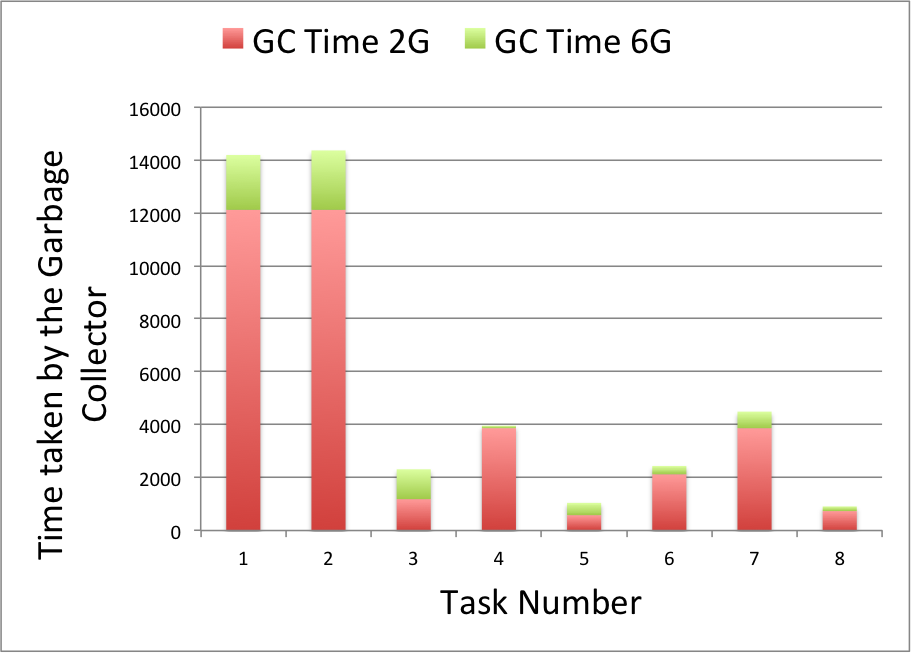
\includegraphics[scale=0.50]{./images/image1.png}
\end{figure}

\paragraph{}
Another observation we have is that the abstraction of RDDs is still
inept when handling search queries on semi-structured datasets, such as
log data from applications, page views etc. When filtering a dataset
Spark has to parse all the partitions within a dataset, while the actual
results might be relevant to only a subset of the overall partitions.
Fig \ref{fig:fig2} shows the comparison between Vanilla Spark's
filtering query and an ideal implementation of a set of queries on a
dump from Wikimedia \cite{wikimedia} where we observe that on an average
only 48\% of the total partitions contain relevant results. This was the
primary motivation behind building a range partitioning mechanism on top
of partitions and thereby indexing the data stored in RDDs.

\begin{figure}[!ht]
\caption{Comparison of query runtimes on Vanilla (V-Spark) and an ideal query engine (I-Spark)}
\label{fig:fig2}
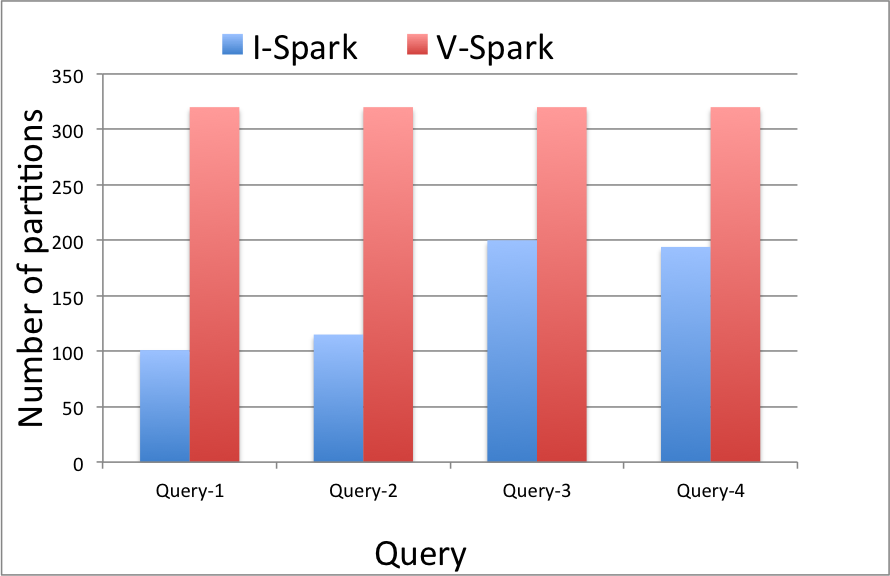
\includegraphics[scale=0.50]{./images/image2.png}
\end{figure}

